\documentclass[nojss]{jss}
\usepackage{thumbpdf}

\author{Ali \"Unl\"u\\University of Augsburg
   \And Thomas Kiefer\\University of Augsburg
   \And Ehtibar N.\ Dzhafarov\\Purdue University}
\Plainauthor{Ali \"Unl\"u, Thomas Kiefer, Ehtibar Dzhafarov}

\title{Fechnerian Scaling in \proglang{R}: The Package \pkg{fechner}}
\Plaintitle{Fechnerian Scaling in R: The Package fechner}

\Abstract{
     This introduction to the \proglang{R} package \pkg{fechner} is based on \cite{Uenlue+Kiefer+Dzhafarov:2009},
     published in the \emph{Journal of Statistical Software}.

     Fechnerian scaling is a procedure for constructing a metric on a set
     of objects (e.g., colors, symbols, X-ray films, or even statistical models)
     to represent dissimilarities among the objects ``from the point of view'' of a system 
     (e.g., person, technical device, or even computational algorithm) ``perceiving'' 
     these objects. This metric, called Fechnerian, is computed from a data matrix 
     of pairwise discrimination probabilities or any other pairwise measure which can be interpreted as the degree 
     with which two objects within the set are discriminated from each other. This paper presents the package
     \pkg{fechner} for performing Fechnerian scaling of object sets in \proglang{R}. We describe the functions
     of the package. Fechnerian scaling then is demonstrated on real and artificial data sets accompanying the package.
}
\Keywords{Fechnerian scaling, psychophysics, metric, subjective dissimilarity, \proglang{R}}
\Plainkeywords{Fechnerian scaling, psychophysics, metric, subjective dissimilarity, R}

\Address{
  Ali \"Unl\"u\\
  Institute of Mathematics\\
  University of Augsburg\\
  D-86135 Augsburg, Germany\\
  E-mail: \email{ali.uenlue@math.uni-augsburg.de}\\
  URL: \url{http://www.math.uni-augsburg.de/~uenlueal/}\\

  Thomas Kiefer\\
  Institute of Mathematics\\
  University of Augsburg\\
  D-86135 Augsburg, Germany\\
  E-mail: \email{thomas.kiefer@student.uni-augsburg.de}\\
  
  Ehtibar N.\ Dzhafarov\\
  Department of Psychological Sciences\\
  Purdue University\\
  West Lafayette, IN 47907-2081, United States of America\\
  E-mail: \email{ehtibar@purdue.edu}\\
  URL: \url{http://www.psych.purdue.edu/~ehtibar/}
}


\begin{document}

\section{Introduction} \label{sec:intro}

This paper discusses the \proglang{R} \citep{R:2009} 
package \pkg{fechner} for Fechnerian scaling (FS) of object (or stimulus) sets. 
It is available from the Comprehensive \proglang{R} Archive Network at
\url{http://CRAN.R-project.org/package=fechner}. See \cite{Uenlue+Kiefer+Dzhafarov:2009}.
FS provides a theoretical framework for deriving so-called Fechnerian distances
among objects from discrimination probabilities or other measures
showing the degree with which objects are discriminated from each
other by what is generically referred to as a perceiving system. In
addition to the Fechnerian distances, FS also identifies pairs of points of subjective equality, 
geodesic chains, and geodesic loops. (These concepts are explained in detail in Section~\ref{sec:FS}.)

This paper provides a brief and by necessity schematic overview of
the main concepts of FS. For detailed discussions of the various developments
in this field refer to the following literature. The latest and most
general version of FS is the dissimilarity cumulation theory \citep{DzhCol2007, Dzh2008a, Dzh2008b}.
This theory extends the previously proposed theories of FS in continuous
\citep{DzhCol2005a} and discrete and discrete-continuous \citep{DzhCol2005b}
stimulus spaces. For historical background and the relation of FS
to traditional issues of psychophysics---for instance, \cite{Fech1860}'s
original theory and its experimental and theoretical critiques---see
\cite{Dzh2001,Dzh2002a,Dzh2002b} and \cite{DzhCol1999,DzhCol2001}.
The finite, discrete version of FS, by far the most important for
practical applications, is discussed in detail in \cite{DzhCol2006b}.
As any data set is necessarily finite, this is the version implemented
in the package \pkg{fechner} and described in the present paper.

\pagebreak

Currently available software for FS includes \pkg{FSCAMDS} \citep{FSCAMDS},
which runs on \proglang{MATLAB} \citep{MATLAB}, and a \proglang{MATLAB} toolbox
\citep{Rach+Colonius:2008}.

The paper is structured as follows. In Section~\ref{sec:FS}, we briefly
review the theory of FS. In Section~\ref{sec:fechner}, we present
the package \pkg{fechner} and describe the functions therein. In
Section~\ref{sec:Ex}, we demonstrate FS by applying the package's
functions to real and artificial data sets accompanying the package.


\section{Fechnerian scaling of object sets}
\label{sec:FS}

Let $\left\{ x_{1},\ldots,x_{n}\right\} $ be a set
of objects endowed with a discrimination function $\psi\left(x_{i},x_{j}\right)$.
The primary meaning of $\psi\left(x_{i},x_{j}\right)$ in FS is the
probability with which $x_{i}$ is judged to be different from (not
the same as) $x_{j}$. For example, a pair of colors $\left(x_{i},x_{j}\right)$
may be repeatedly presented to an observer (or a group of observers),
and $\psi\left(x_{i},x_{j}\right)$ may be estimated by the frequency
of responses ``they are different''. Or $\left(x_{i},x_{j}\right)$
may be a pair of categories, and $\psi\left(x_{i},x_{j}\right)$ the
frequency of times a randomly chosen exemplar of category $x_{i}$
and a randomly chosen exemplar of category $x_{j}$ are judged by
a person to belong to different categories. Or $\left(x_{i},x_{j}\right)$
may be a pair of statistical models, and $\psi\left(x_{i},x_{j}\right)$
the probability with which model $x_{j}$ fails to fit
(by some statistical criterion) a randomly chosen data set generated
by model $x_{i}$. Possible examples are numerous, and more can be
found in \cite{DzhCol2006a}. If warranted by substantive considerations,
$\psi\left(x_{i},x_{j}\right)$ may represent nonlinearly transformed
probabilities, such as their logarithms or inverse normal integrals.
Moreover, $\psi$ need not be related to probabilities at all: one
can, for example, repeatedly present a pair of colors $\left(x_{i},x_{j}\right)$
and ask an observer for a direct numerical estimate of {}``how dissimilar
$x_{i}$ and $x_{j}$ are'' (say, on a scale from $0$ to $10$), in which
case $\psi\left(x_{i},x_{j}\right)$ can be the median or mean of
several numerical estimates \citep[this procedure is commonly used for the
purposes of multidimensional scaling, MDS; see, e.g.,][]{KruskWish1978}.

It is a well-established empirical fact that $\psi\left(x_{i},x_{j}\right)$,
however obtained, is not a metric:
\begin{itemize}
\item [(1)] $\psi\left(x_{i},x_{i}\right)$ is not always zero;
\item [(2)] moreover, $\psi\left(x_{i},x_{i}\right)$ and $\psi\left(x_{j},x_{j}\right)$
for $i\neq j$ are not generally the same;
\item [(3)] $\psi\left(x_{i},x_{j}\right)$ is generally different from
$\psi\left(x_{j},x_{i}\right)$;
\item [(4)] and the triangle inequality is not generally satisfied either,
$\psi\left(x_{i},x_{j}\right)+\psi\left(x_{j},x_{k}\right)$ may very
well be less than $\psi\left(x_{i},x_{k}\right)$.
\end{itemize}
The only data-analytic procedure other than FS which is aimed at imposing
a metric on $\left\{ x_{1},\ldots,x_{n}\right\} $ based on $\psi$
is nonmetric MDS \citep[e.g.,][]{KruskWish1978}. 
In its common version MDS assumes that $\psi\left(x_{i},x_{j}\right)$
is some unknown monotone transformation of a ``true'' distance
$d\left(x_{i},x_{j}\right)$, and the MDS procedure searches for this
transformation. No transformation, however, can deal with points (2)
and (3) above, so the data have to be modified to make MDS applicable:
e.g., $\psi\left(x_{i},x_{j}\right)$ and $\psi\left(x_{j},x_{i}\right)$
are replaced with their averages, and all ``diagonal'' values
$\psi\left(x_{i},x_{i}\right)$ are averaged over as well. Even then
MDS may not succeed in finding the transformation, 
especially since the class of allowable metrics in MDS is usually a priori
restricted to Euclidean (or so-called Minkowskian) metrics in low-dimensional
spaces of real-component vectors.

By contrast, FS deals directly with $\psi$-data subject to points
1--4 above, and it imposes no a priori restrictions on the class of
metrics $d$ computed from $\psi$. The only property of the $\psi$-data
which is required by FS is regular minimality (RM).
This property can be formulated in three statements:
\begin{itemize}
\item [(A)] for every $x_{i}$ there is one and only one $x_{j}$ such
that $\psi\left(x_{i},x_{j}\right)<\psi\left(x_{i},x_{k}\right)$
for all $k\neq j$ (this $x_{j}$ is called the Point of Subjective
Equality, or PSE, of $x_{i}$);
\item [(B)] for every $x_{j}$ there is one and only one $x_{i}$ such
that $\psi\left(x_{i},x_{j}\right)<\psi\left(x_{k},x_{j}\right)$
for all $k\neq i$ (this $x_{i}$ is called the PSE of $x_{j}$);
\item [(C)] and $x_{j}$ is the PSE of $x_{i}$ if and only if $x_{i}$
is the PSE of $x_{j}$.
\end{itemize}
Every data matrix in which the diagonal entry $\psi\left(x_{i},x_{i}\right)$
is smaller than all entries $\psi\left(x_{i},x_{k}\right)$ in its
row ($k\neq i)$ and all entries $\psi\left(x_{k},x_{i}\right)$ in
its column ($k\neq i)$ satisfies RM in the simplest (so-called canonical) form. 
In this simplest case every object $x_{i}$ is the PSE of $x_{i}$. 
(Note that regular maximality can be defined analogously, 
replacing ``minimal'' with ``maximal''.
This is required when the $\psi$-data represent closeness values rather than differences; e.g., 
$\psi\left(x_{i},x_{j}\right)$ may be the percent of times $x_{i}$ is judged to be the same as 
$x_{j}$.)

It need not always be the case, however, that every $x_{i}$ is the PSE of $x_{i}$.
What makes any $\left(x_{i},x_{j}\right)$ an ordered pair, different from $\left(x_{j},x_{i}\right)$,
and what makes $\left(x_{i},x_{i}\right)$ a pair rather than a single
object, is the fact that $x_{i}$ and $x_{j}$ (in particular, $x_{i}$ and $x_{i}$),
when being compared, necessarily differ in some property which ``does
not count'' for the comparison. For example, if $x_{i}$ and $x_{j}$
are two colors, they must occupy two different spatial locations,
or one of them may be presented first and the other second in time.
This difference in spatial or temporal locations (generically referred to as the difference between two observation areas) 
does not enter in the comparison, but it may affect the way people perceive colors, and
this in turn may lead to $\psi\left(x_{i},x_{i}\right)$ being larger
than $\psi\left(x_{i},x_{j}\right)$ for some distinct $i$ and $j$
(in the same way as it may lead to $\psi\left(x_{i},x_{j}\right)\neq\psi\left(x_{j},x_{i}\right)$).
The matrix of $\psi$-data
\[
\left[\begin{array}{cccc}
 & x_{1} & x_{2} & x_{3}\\
x_{1} & 0.2 & 0.1 & 0.5\\
x_{2} & 0.7 & 0.3 & 0.2\\
x_{3} & 0.1 & 0.6 & 0.3\end{array}\right]
\]
satisfies RM, with $\left(x_{1},x_{2}\right)$, $\left(x_{2},x_{3}\right)$,
and $\left(x_{3},x_{1}\right)$ being pairs of mutual PSEs. Here,
the first symbol in every pair refers to a row object (all row objects belonging to one, the ``first'', observation area) 
and the second symbol refers to a column object (in the ``second'' observation area).

Generalizing, given a matrix of $\psi\left(x_{i},x_{j}\right)$-values
with the rows and columns labeled by the objects $\left\{ x_{1},\ldots,x_{n}\right\}$,
if (and only if) RM is satisfied, the row objects and column objects
can be presented in pairs of PSEs $\left(x_{1},x_{k_{1}}\right),\left(x_{2},x_{k_{2}}\right),\ldots,\left(x_{n},x_{k_{n}}\right)$,
where $\left(k_{1},k_{2},\ldots,k_{n}\right)$ is a permutation of
$\left(1,2,\ldots,n\right)$. The FS procedure identifies and lists
these PSE pairs and then relabels them so that two members of the
same pair receive one and the same label: 
\[
\left(x_{1},x_{k_{1}}\right)\mapsto\left(a_{1},a_{1}\right),\left(x_{2},x_{k_{2}}\right)\mapsto\left(a_{2},a_{2}\right),\ldots,\left(x_{n},x_{k_{n}}\right)\mapsto\left(a_{n},a_{n}\right).
\]
Thus, the matrix in the example above becomes
\[
\left[\begin{array}{cccc}
 & a_{3} & a_{1} & a_{2}\\
a_{1} & 0.2 & 0.1 & 0.5\\
a_{2} & 0.7 & 0.3 & 0.2\\
a_{3} & 0.1 & 0.6 & 0.3\end{array}\right]=\left[\begin{array}{cccc}
 & a_{1} & a_{2} & a_{3}\\
a_{1} & 0.1 & 0.5 & 0.2\\
a_{2} & 0.3 & 0.2 & 0.7\\
a_{3} & 0.6 & 0.3 & 0.1\end{array}\right]
\]
in which each diagonal entry is minimal in its row and in its column.
After this relabeling the original function $\psi\left(x_{i},x_{j}\right)$
is redefined. We present it as $p_{ij}=\hat{\psi}(a_i,a_j)$ according to the rule: if
$\left(x_{i},x_{k_{i}}\right)\mapsto\left(a_{i},a_{i}\right)$ and
$\left(x_{j},x_{k_{j}}\right)\mapsto\left(a_{j},a_{j}\right)$, then
$p_{ij}=\psi\left(x_{i},x_{k_{j}}\right)$ (in particular, $p_{ii}=\psi\left(x_{i},x_{k_{i}}\right)$).
Note that $p_{ij}$ is subject to the same properties 1--4 which were
stipulated above for $\psi$. Of course, in the simplest case (canonical form), when
each $x_{i}$ is its own PSE, no relabeling of objects is necessary,
and $p_{ij}$ coincides with $\psi\left(x_{i},x_{j}\right)$. (In the package \pkg{fechner}
the pairs of PSEs are assigned identical labels leaving intact the labeling of the rows 
and relabeling the columns with their corresponding PSEs. 
This is referred to as canonical relabeling.)

FS imposes a metric $G$ on the set $\left\{ a_{1},\ldots,a_{n}\right\}$
in such a way that, if $x_{i}$ and $x_{i'}$ are each other's PSEs
relabeled into $a_{i}$ and $x_{j}$ and $x_{j'}$ are each other's
PSEs relabeled into $a_{j}$, then $G\left(x_{i},x_{j}\right)=G\left(x_{i'},x_{j'}\right)=G\left(a_{i},a_{j}\right)$.
Here is how it is done. Let any finite sequence of objects, not necessarily pairwise distinct, be called a chain. 
Any ordered pair of successive objects in a chain 
is referred to as a link of the chain.
For every pair of objects $\left(a_{i},a_{j}\right)$
we consider all possible chains of objects $\left(a_{i},a_{k_{1}},\ldots,a_{k_{r}},a_{j}\right)$,
where $\left(a_{k_{1}},\ldots,a_{k_{r}}\right)$ is a sequence chosen
from $\left\{ a_{1},\ldots,a_{n}\right\} $ (and $r$ may be $0$, in
which case the chain inserted between $a_{i}$ and $a_{j}$ is empty).
For each such a chain we compute what is called its psychometric length (of the first kind) as
\[
L^{(1)}\left(a_{i},a_{k_{1}},\ldots,a_{k_{r}},a_{j}\right)=\sum_{m=0}^{m=r}\left(p_{k_{m}k_{m+1}}-p_{k_{m}k_{m}}\right),
\]
where we put $a_{i}=a_{k_{0}}$ and $a_{j}=a_{k_{r+1}}$. (The quantities $p_{k_{m}k_{m+1}}-p_{k_{m}k_{m}}$
are referred to as psychometric increments of the first kind.)
Then we find a chain (which need not be unique) with the minimal value of
$L^{(1)}$, and take this minimal value of $L^{(1)}$ for the quasidistance
$G_{ij}^{(1)}$ from $a_{i}$ to $a_{j}$ (referred to as the oriented Fechnerian distance of the first kind). 
Quasidistance (quasimetric, or oriented metric) is a pairwise measure which satisfies all metric properties 
except for symmetry: $G_{ij}^{(1)}=0$ if and only if $i=j$,
and $G_{ij}^{(1)}+G_{jk}^{(1)}\geq G_{ik}^{(1)}$, but $G_{ij}^{(1)}$
need not equal $G_{ji}^{(1)}$. 
(The proof that $G_{ij}^{(1)}$ is a quasidistance is straightforward. See \cite{DzhCol2007}
for the most general version.) 
In FS we symmetrize this quasimetric and transform it into a metric by computing $G_{ij}^{(1)}+G_{ji}^{(1)}$
and taking it for the ``true'' or ``overall'' Fechnerian distance $G_{ij}$
between $a_{i}$ and $a_{j}$. Any chain $\left(a_{i},a_{k_{1}},\ldots,a_{k_{r}},a_{j}\right)$
with $L^{(1)}\left(a_{i},a_{k_{1}},\ldots,a_{k_{r}},a_{j}\right)=G_{ij}^{(1)}$
is called a geodesic chain (of the first kind). Then the overall Fechnerian distance $G_{ij}$ (see Figure~\ref{fig:1}) 
is the psychometric length (of the first kind) of a geodesic loop $\left(a_{i},a_{k_{1}},\ldots,a_{k_{r}},a_{j},a_{l_{1}},\ldots,a_{l_{s}},a_{i}\right)$,
or equivalently $\left(a_{j},a_{l_{1}},\ldots,a_{l_{s}},a_{i},a_{k_{1}},\ldots,a_{k_{r}},a_{j}\right)$.  

\begin{figure}[t!]
\begin{center}
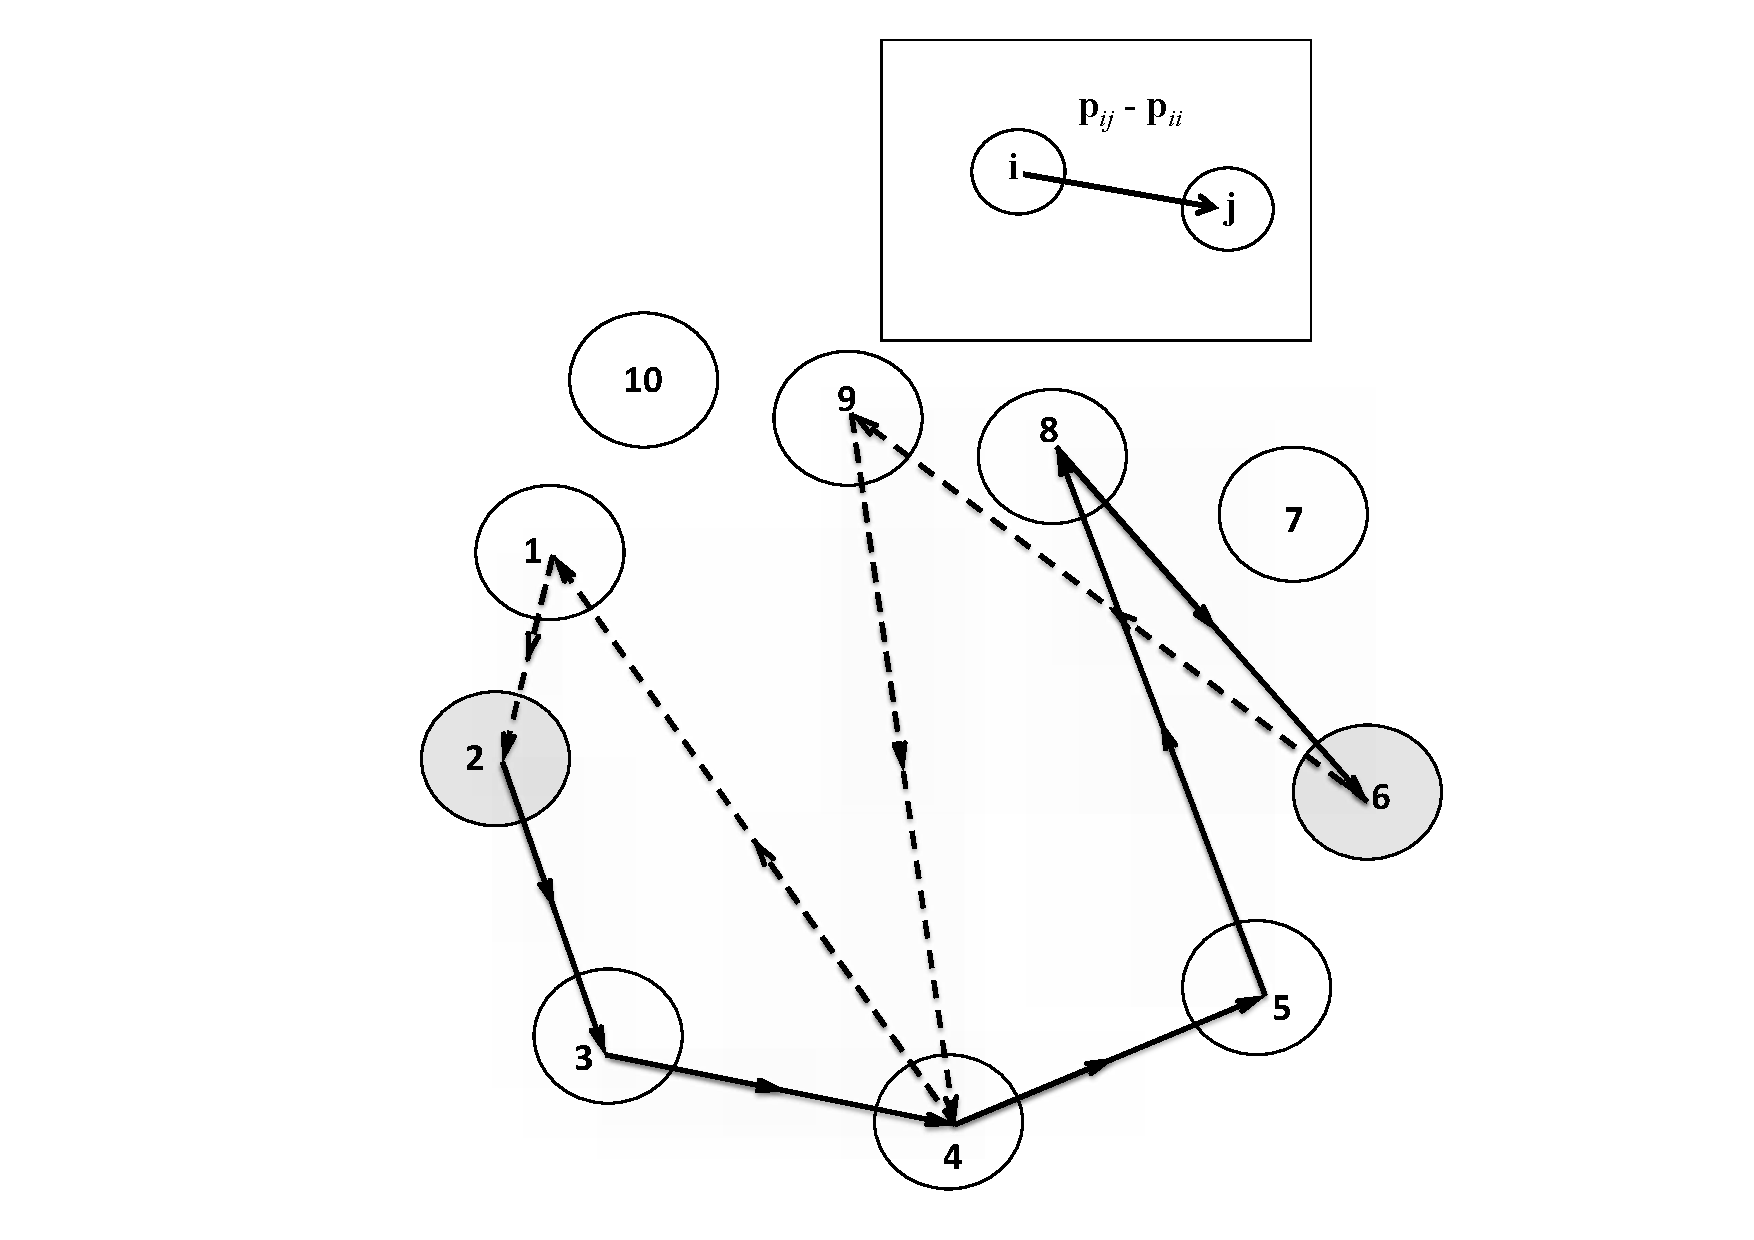
\includegraphics[scale=1]{fig1.pdf}
\caption{A space consisting of $10$ objects shown in an arbitrary spatial
arrangement. The psychometric length (of the first kind) $L^{(1)}\left(2,3,4,5,8,6\right)$
of the chain connecting object $2$ to object $6$ (shown by solid arrows, representing the links of the chain)
is computed as $\left(p_{23}-p_{22}\right)+\left(p_{34}-p_{33}\right)+\left(p_{45}-p_{44}\right)+\left(p_{58}-p_{55}\right)+\left(p_{86}-p_{88}\right)$.
If this chain is the shortest among all chains connecting object $2$
to object $6$, then $L^{(1)}\left(2,3,4,5,8,6\right)$ is
taken to be the oriented Fechnerian distance $G_{26}^{(1)}$ from
$2$ to $6$. Analogously, $L^{(1)}\left(6,9,4,1,2\right)$ of
the chain connecting object $6$ to object $2$ (shown by dashed arrows, representing the links of the chain)
is $\left(p_{69}-p_{66}\right)+\left(p_{94}-p_{99}\right)+\left(p_{41}-p_{44}\right)+\left(p_{12}-p_{11}\right)$.
If this chain is the shortest among all chains connecting object $6$
to object $2$, then $L^{(1)}\left(6,9,4,1,2\right)=G_{62}^{(1)}$.
Together the two chains form a loop with the total length $L^{(1)}\left(2,3,4,5,8,6\right)+L^{(1)}\left(6,9,4,1,2\right)$.
If the two chains are the shortest possible, then this sum is the
overall Fechnerian distance $G_{26}=G_{62}$ between objects $2$ and $6$.}
\label{fig:1}
\end{center}
\end{figure}  

Although this is not, strictly speaking, necessary for computations,
it is worth noting that we can also compute the psychometric length (of the second kind) of an arbitrary
chain $\left(a_{i},a_{k_{1}},\ldots,a_{k_{r}},a_{j}\right)$ as
\[
L^{(2)}\left(a_{i},a_{k_{1}},\ldots,a_{k_{r}},a_{j}\right)=\sum_{m=0}^{m=r}\left(p_{k_{m+1}k_{m}}-p_{k_{m}k_{m}}\right)
\]
(where $p_{k_{m+1}k_{m}}-p_{k_{m}k_{m}}$ are called psychometric increments of the second kind), and then define the quasidistance 
(the oriented Fechnerian distance of the second kind) $G_{ij}^{(2)}$ from $a_{i}$ to $a_{j}$ as the minimal value of $L^{(2)}$ 
across all chains inserted between $a_{i}$ and $a_{j}$. It makes, however, no difference
for the final computation of the overall Fechnerian distance $G_{ij}$, because
it can be shown \citep[see, e.g.,][]{DzhCol2006b} that 
\[
G_{ij}=G_{ij}^{(1)}+G_{ji}^{(1)}=G_{ij}^{(2)}+G_{ji}^{(2)}.
\]
It also holds (in fact, the equality above is an immediate consequence of this result) that the $L^{(1)}$--length 
of any loop $\left(a_{i},a_{k_{1}},\ldots,a_{k_{r}},a_{j},a_{l_{1}},\ldots,a_{l_{s}},a_{i}\right)$
equals the $L^{(2)}$--length of the same loop traversed in the opposite direction, 
$\left(a_{i},a_{l_{s}},\ldots,a_{l_{1}},a_{j},a_{k_{r}},\ldots,a_{k_{1}},a_{i}\right)$; 
see Figure~\ref{fig:2}.

\begin{figure}[t!]
\begin{center}
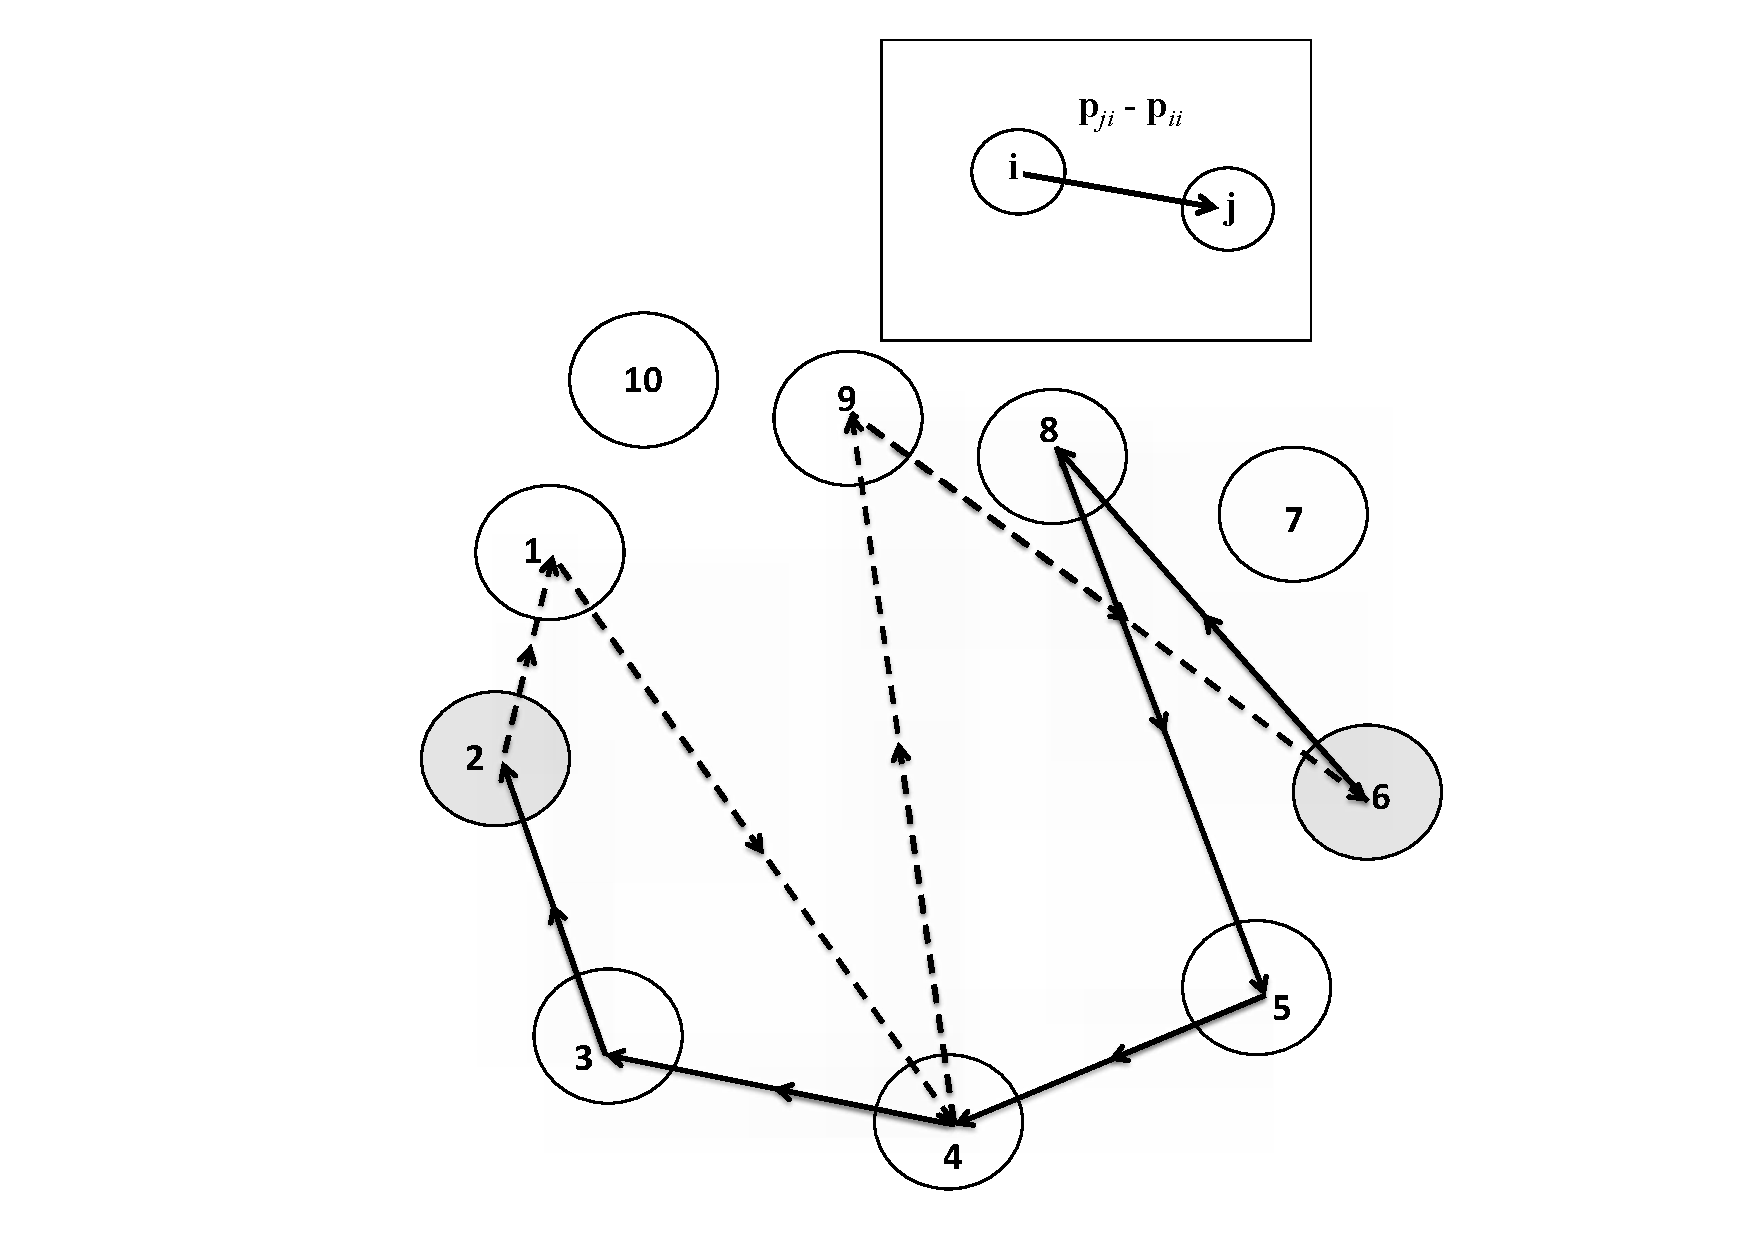
\includegraphics[scale=1]{fig2.pdf}
\caption{The same as Figure~\ref{fig:1}, but the loop comprised of the solid
and dashed arrows (representing the links of the loop) is now traversed in the opposite direction. The
psychometric length (of the second kind) $L^{(2)}\left(6,8,5,4,3,2\right)$
is computed as $\left(p_{86}-p_{66}\right)+\left(p_{58}-p_{88}\right)+\left(p_{45}-p_{55}\right)+\left(p_{34}-p_{44}\right)+\left(p_{23}-p_{33}\right)$.
Analogously, $L^{(2)}\left(2,1,4,9,6\right)$ is $\left(p_{12}-p_{22}\right)+\left(p_{41}-p_{11}\right)+\left(p_{94}-p_{44}\right)+\left(p_{69}-p_{99}\right)$.
It can be verified by rearranging terms that the length
$L^{(2)}\left(6,8,5,4,3,2\right)+L^{(2)}\left(2,1,4,9,6\right)$
of this loop is the same as the length of the loop computed in Figure~\ref{fig:1}: 
$L^{(1)}\left(2,3,4,5,8,6\right)+L^{(1)}\left(6,9,4,1,2\right)$.
As a consequence, if the loop in Figure~\ref{fig:1} is the shortest in the $L^{(1)}$ sense among all
loops containing objects $2$ and $6$, then so is in the $L^{(2)}$ sense the loop traversed in
the opposite direction (and vice versa); hence $G_{26}^{(1)}+G_{62}^{(1)}=G_{26}^{(2)}+G_{62}^{(2)}=G_{26}$,
the overall Fechnerian distance between objects $2$ and $6$.}
\label{fig:2}
\end{center}
\end{figure}  

The package \pkg{fechner} computes, among other quantities (see Section~\ref{sec:fechner}), the value of $G_{ij}$ 
(referred to as $G$ in the package) and identifies
a geodesic loop (perhaps one of several possible) for any pair of
(relabeled) objects $\left(a_{i},a_{j}\right)$. It also compares
the value of $G_{ij}$ to what we call a generalized Shepardian index of dissimilarity
$S_{ij}=p_{ij}+p_{ji}-p_{ii}-p_{jj}$ (referred to as $S$--index in the package).\footnote{Shepard's original index, 
in our notation, is $S_{ij}^{*}=\left(\left(1-p_{ij}\right)\left(1-p_{ji}\right)\right)/\left(\left(1-p_{ii}\right)\left(1-p_{jj}\right)\right)$
\citep[][]{Shepard1957, Shepard1987}. In FS $S_{ij}$ is called the generalized Shepardian index 
because it achieves the same goal as $S_{ij}^{*}$: it symmetrizes the matrix about the main diagonal and equalizes 
all diagonal entries (although their common value in $S_{ij}^{*}$ is $1$ rather than $0$).
The index $S_{ij}^{*}$ can be viewed as a special case of $S_{ij}$ if $p$ in $S_{ij}$ is understood as 
$\log\left(1-p\right)$ in $\log S_{ij}^{*}$.}
Note that $G_{ij}\leq S_{ij}$ for all $\left(a_{i},a_{j}\right)$. 
The comparison $G_{ij}$ versus $S_{ij}$ is of interest because it shows how different the psychometric increments 
$p_{ij}-p_{ii}$ are from an oriented metric.
The equality $G_{ij}=S_{ij}$ holds for some $\left(a_{i},a_{j}\right)$ if and only if the geodesic loop for
$\left(a_{i},a_{j}\right)$ contains no other objects, i.e., if it is $\left(a_{i},a_{j},a_{i}\right)$. 
This means that $p_{ij}-p_{ii}$ is smaller than $L^{(1)}\left(a_{i},a_{k_{1}},\ldots,a_{k_{r}},a_{j}\right)$
for any chain inserted between $a_{i}$ and $a_{j}$, and that $p_{ji}-p_{jj}$ is smaller than $L^{(1)}\left(a_{j},a_{l_{1}},\ldots,a_{l_{s}},a_{i}\right)$
for any chain inserted between $a_{j}$ and $a_{i}$. (The same statement could be equivalently formulated in terms of psychometric increments
and lengths of the second kind, $p_{ji}-p_{ii}$ and $L^{(2)}$.)
It follows that if $G_{ij}=S_{ij}$ for all $\left(a_{i},a_{j}\right)$, then the values of $p_{ij}-p_{ii}$ form an oriented metric, and the computation
of $G_{ij}$ is reduced to simple symmetrization: $\left(p_{ij}-p_{ii}\right)+\left(p_{ji}-p_{jj}\right)=S_{ij}$.
The greater the number of points $\left(a_{i},a_{j}\right)$ for which $G_{ij}<S_{ij}$ and the greater the differences $S_{ij}-G_{ij}$, 
the greater the ``non-metricality'' of the psychometric increments $p_{ij}-p_{ii}$ and the greater the ``improvement'' they need to become metric. 
To quantify this ``improvement'' FS uses an ad hoc descriptive index
\[
C=\frac{2\sum\left(S_{ij}-G_{ij}\right)^{2}}{\sum S_{ij}^{2}+\sum G_{ij}^{2}}
\]
(referred to as $C$--index in the package).

\section[The R package fechner]{The \proglang{R} package \pkg{fechner}}
\label{sec:fechner}

In this section we briefly describe the functions and relevant parts of the package. 
How to actually use the software is demonstrated on examples in Section~\ref{sec:Ex}.
The description of the package will be short, primarily focusing on the main aspects of FS, those the users may want to know first. 
Detailed information about these and other matters can be found in the comprehensive documentation files
for the package in \proglang{R}. We do not discuss source code because the code in \pkg{fechner} is straightforward, intuitive, 
and generously commented.

The package \pkg{fechner} is implemented based on the \proglang{S}3 system.  
It comes with a namespace and consists of three external functions (functions the package exports):
the main function \code{fechner}, which provides the FS computations, and the functions \code{check.regular} 
and \code{check.data} for verifying the required regular minimality/maximality property and the format of the data, 
respectively. The package also contains internal functions (functions not exported by the package), which basically 
are \code{plot}, \code{print}, and \code{summary} methods for objects of the class ``\code{fechner}''.
There are two real and two artificial data sets accompanying the package \pkg{fechner} 
(they are described and analyzed in Section~\ref{sec:Ex}).
The package's functionality and output closely follow that of the software \pkg{FSCAMDS} (see Section~\ref{sec:intro}). 
It was tested on real and artificial data and yielded the same results 
as obtained with \pkg{FSCAMDS}.
Detailed descriptions of the package's functions and data sets can be found in the documentation
files in \proglang{R} (for an overview, type \code{package?fechner}).

The main function of the package is \code{fechner}: 
\begin{Code}
fechner(X, format = c("probability.different", "percent.same", "general"), 
  compute.all = FALSE, check.computation = FALSE)
\end{Code}
This function provides the FS computations (see Section~\ref{sec:FS}), in two variants, termed ``short'' and ``long''. 
The short computation (\code{compute.all = FALSE}) returns a list, of the class ``\code{fechner}'', 
containing such information as the pairs of PSEs, the canonical representation of the data 
in which regular minimality/maximality is satisfied in the canonical form and the rows and columns are canonically relabeled, 
the $S$--index, and most importantly, the overall Fechnerian distances and geodesic loops. 
The long computation (\code{compute.all = TRUE}) additionally yields intermediate results, 
such as the psychometric increments, the oriented Fechnerian distances, and the geodesic chains, 
and it also allows to check the equality
\[
\left(G_{ij}^{(1)}+G_{ji}^{(1)}\right) - \left(G_{ij}^{(2)}+G_{ji}^{(2)}\right) = 0
\]
(\code{check.computation = TRUE}). This equality must hold by theory (see Section~\ref{sec:FS}).

The function \code{fechner} takes a square matrix or a data frame of numeric data (\code{X}; e.g., discrimination probabilities), 
which must be in one of the following formats: probability-different, percent-same, or general. 
The data have to be a matrix or a data frame with the same number of rows and columns, and the data have to be numeric 
(no infinite, undefined, or missing values are allowed). This is the general data format. 
The probability-different and percent-same formats, in addition, require that the data lie in the intervals $[0, 1]$ and $[0, 100]$, respectively. 
In the percent-same format, the data are automatically transformed prior to the analysis using the transformation $(100 - X) / 100$. 

The only property of the data which is required by FS is regular minimality/maximality (see Section~\ref{sec:FS}). 
For the percent-same format the data must satisfy regular maximality, for the probability-different and general formats, regular minimality. 
This property can be checked using the function \code{check.regular}:
\begin{Code}
check.regular(X, type = c("probability.different", "percent.same",
  "reg.minimal", "reg.maximal"))
\end{Code}
This function takes a square matrix or a data frame of numeric data (\code{X}; see \code{fechner} above) and returns a list consisting 
of the canonical representation of the data, 
the pairs of PSEs, a character string saying which check was performed (regular minimality or regular maximality),
and a logical indicating whether the original data are already in the canonical form. The values \code{"reg.minimal"} and \code{"reg.maximal"} can be specified 
to force checking for regular minimality and regular maximality, respectively, independent of the data set used.

The data format can be checked using the function \code{check.data}:
\begin{Code}
check.data(X, format = c("probability.different", "percent.same", "general"))
\end{Code}
This function takes a square matrix or a data frame of numeric data (\code{X}; see \code{fechner} above) 
and returns a matrix of the data with rows and columns labeled. The labeling is as follows:
\begin{itemize}
\item If the data are entered without any labeling of the rows and columns, \code{check.data} does the labeling automatically: as
$a1, b1, \ldots, z1$, $a2, b2, \ldots, z2$, etc., up to $a9, b9, \ldots, z9$ 
if the data size does not exceed $234\times 234$, or if the data size is larger than $234\times 234$, 
the labeling is $v1, v2, \ldots, vN$, where $N\times N$ is the dimensionality of the data 
(and $N > 234$).
\item If the data are entered with either row or column labeling (but not both), the row or column labels are assigned
to the columns or rows, respectively.
\item If the data are entered with row and column labeling, the same labeling must be used for both. If this is the
case, the labeling is adopted. 
\end{itemize}

The interdependencies among these three functions of the package are as follows. 
The function \code{fechner} calls the function \code{check.regular}, which in turn calls \code{check.data}.  In particular, in the function \code{fechner}
the specified data format and regular 
minimality/maximality are checked, and the rows and columns of the canonical representation matrix are canonically relabeled 
based on the labeling provided by \code{check.data}. 
That is, using the \code{check.data} labeling, the pairs of PSEs are assigned identical labels leaving intact the labeling of the rows and relabeling the 
columns with their corresponding PSEs (see Section~\ref{sec:FS}).

The function \code{fechner} returns an object (\code{x} or \code{object}) of the class ``\code{fechner}'', 
for which \proglang{S}3 \code{plot}, \code{print}, and \code{summary} methods are provided.
The \code{plot} method 
\begin{Code}
plot(x, level = 2)
\end{Code}
graphs the results obtained in the FS analyses. It produces a scatterplot of the overall Fechnerian distance $G$ versus the $S$--index
(for off-diagonal pairs of stimuli/objects), with rugs added to the axes and jittered (\code{amount = 0.01} of noise) to accommodate ties in the $S$--index and $G$ values. 
The diagonal line $y = x$ is provided for a visual reference in estimating the differences between the two types of values, as a measure of ``non-metricality'' 
of the psychometric increments (see Section~\ref{sec:FS}).
The level of comparison (an integer greater than or equal to $2$) refers to the minimum number of links in geodesic loops for the pairs of stimuli considered for the comparison.
That is, choosing level $n$ means that the comparison involves only those $S$--index and $G$ values that correspond to the geodesic loops 
containing not less than $n$ links. Normally the differences between the $S$--index and $G$ values are greater for pairs of objects
having geodesic loops with more links (see Figures~\ref{fig:3} and \ref{fig:4}).
The \code{print} method 
\begin{Code}
print(x)
\end{Code}
prints the main results obtained in the FS analyses, which are the overall Fechnerian distances 
and the geodesic loops. 
The \code{summary} method 
\begin{Code}
summary(object, level = 2)
\end{Code}
outlines the results obtained in the FS analyses. It returns a list  
consisting of the pairs of objects and their corresponding $S$--index and $G$ values, the value of the Pearson correlation coefficient between them,
the value of the $C$--index (as an ad hoc measure of the ``improvement'' the psychometric increments need to become metric; 
see Section~\ref{sec:FS}), and the level of comparison chosen. 
Detailed summary information such as individual object pairs and their 
corresponding $S$--index and $G$ values can be accessed through assignment.
(Note that the \code{summary} method returns an object of the class ``\code{summary.fechner}'', 
for which a \code{print} method is provided.)


\section{Examples}
\label{sec:Ex}

The package \pkg{fechner} contains two real (\code{morse} and \code{wish}) and two artificial (\code{regMin} and \code{noRegMin})
data sets. We use these data sets to demonstrate the functions of the package. 

\subsection{The data sets}

\code{morse}: \cite{Rothk1957}'s Morse code data of discrimination probabilities among $36$ auditory Morse code signals for the letters 
$A, B, \ldots, Z$ and the digits $0, 1, \ldots, 9$. The \code{morse} data frame consists of $36$ rows and $36$ columns, representing 
the Morse code signals presented first and second, respectively. Each number, 
an integer, in the data frame gives the percentage of subjects who responded
``same'' (choosing between ``same'' and ``different'') to the row signal followed by the column signal. 
Each signal consists of a sequence of dots and dashes. A chart of
the Morse code letters and digits can be found in \cite{Wiki+Morse:2009}.

\code{wish}: \cite{Wish1967}'s Morse-code-like data of discrimination probabilities among $32$ auditory Morse-code-like signals. 
The \code{wish} data frame consists of $32$ rows and $32$ columns, representing the Morse-code-like signals presented first and second, respectively. 
Each number, a numeric, in the data frame gives the relative frequency of subjects who responded ``different'' (choosing between ``same'' and ``different'') 
to the row signal followed by the column signal. 
The $32$ Morse-code-like signals in \cite{Wish1967}'s study were $5$-element sequences $T_1P_1T_2P_2T_3$, 
where $T$ stands for a tone (short or long) and $P$ stands for a pause ($1$ or $3$ units long). The stimuli are labeled 
$A, B, \ldots, Z, 0, 1, \ldots, 5$, in the order they are presented in \cite{Wish1967}'s article.

\code{regMin} and \code{noRegMin}: Artificial data of fictitious discrimination probabilities among $10$ stimuli. 
The \code{regMin} and \code{noRegMin} data frames consist of $10$ rows and $10$ columns, representing the fictitious stimuli presented in the first 
and second observation area, respectively.  Each number, a numeric, in the data frames is assumed to give the relative frequency of 
perceivers responding ``different'' to the row stimulus followed by the column stimulus. These artificial data sets are included as examples of a case when regular
minimality holds in the non-canonical form (\code{regMin}) and a case when regular minimality is violated (\code{noRegMin}). 
They differ only in one entry: in the ninth row and the tenth column.

\subsection{Checking data format and regular minimality/maximality}
\label{subsec:regmin}

The data set \code{morse} is in the percent-same format, the \code{wish} data set is in the probability-different format (the \proglang{R} output is omitted,
for typographic reasons):
\begin{CodeChunk}
\begin{CodeInput}
R> check.data(morse, format = "percent.same")
R> check.data(wish, format = "probability.different")
\end{CodeInput}
\end{CodeChunk}

The following code describes an example matrix without labeling of the rows and columns, in the general format; 
\code{check.data} does the labeling automatically:
\begin{CodeChunk}
\begin{CodeInput}
R> (X <- ((-1) * matrix(1:16, nrow = 4)))
\end{CodeInput}
\begin{CodeOutput}
     [,1] [,2] [,3] [,4]
[1,]   -1   -5   -9  -13
[2,]   -2   -6  -10  -14
[3,]   -3   -7  -11  -15
[4,]   -4   -8  -12  -16
\end{CodeOutput}
\begin{CodeInput}
R> check.data(X, format = "general")
\end{CodeInput}
\begin{CodeOutput}
   a1 b1  c1  d1
a1 -1 -5  -9 -13
b1 -2 -6 -10 -14
c1 -3 -7 -11 -15
d1 -4 -8 -12 -16
\end{CodeOutput}
\end{CodeChunk}

\pagebreak

The data set \code{wish} satisfies regular minimality in the canonical form:
\begin{CodeChunk}
\begin{CodeInput}
R> check.regular(wish)$check
\end{CodeInput}
\begin{CodeOutput}
[1] "regular minimality"
\end{CodeOutput}
\begin{CodeInput}
R> check.regular(wish)$in.canonical.form
\end{CodeInput}
\begin{CodeOutput}
[1] TRUE
\end{CodeOutput}
\end{CodeChunk}

The data set \code{morse} satisfies regular maximality in the canonical form:
\begin{CodeChunk}
\begin{CodeInput}
R> check.regular(morse, type = "percent.same")$check
\end{CodeInput}
\begin{CodeOutput}
[1] "regular maximality"
\end{CodeOutput}
\begin{CodeInput}
R> check.regular(morse, type = "percent.same")$in.canonical.form
\end{CodeInput}
\begin{CodeOutput}
[1] TRUE
\end{CodeOutput}
\end{CodeChunk}

For typographic reasons only, in the remainder we consider small subsets of these stimulus sets, chosen to form ``self-contained'' 
subspaces: a geodesic loop for any two elements of such a subset (computed using the complete data set) is contained entirely 
within the subset. (Note that the results obtained in the FS analyses restricted to self-contained subspaces are the same 
as the results obtained from the entire stimulus sets. See below.) 
For instance, a particular self-contained $10$-code subspace of the $36$ Morse codes consists of the codes for the letter $B$ 
and the digits $0, 1, 2, 4, 5, \ldots, 9$.
\begin{CodeChunk}
\begin{CodeInput}
R> indices <- which(is.element(names(morse), c("B", c(0, 1, 2, 4:9))))
R> f.scal.morse <- fechner(morse, format = "percent.same")
R> f.scal.morse$geodesic.loops[indices, indices]
\end{CodeInput}
\begin{CodeOutput}
        B    1     2    4    5      6      7       8      9      0
B       B  B1B   B2B B46B  B5B    B6B  B676B B67876B B6789B   B06B
1     1B1    1   121  141  151    161   1781     181    191    101
2     2B2  212     2  242  252    262    272     282   2192  21092
4    46B4  414   424    4  454   46B4    474    4784    494    404
5     5B5  515   525  545    5   56B5    575     585    595    505
6     6B6  616   626 6B46 6B56      6    676   67876 678976    606
7   76B67 7817   727  747  757    767      7     787   7897 789097
8 876B678  818   828 8478  858  87678    878       8    898   8908
9  9B6789  919  9219  949  959 976789   9789     989      9    909
0    06B0  010 09210  040  050    060 097890    0890    090      0
\end{CodeOutput}
\end{CodeChunk}

This part of the \code{morse} data satisfies regular maximality in the canonical form:
\begin{CodeChunk}
\begin{CodeInput}
R> (morse.subspace <- morse[indices, indices])
\end{CodeInput}
\begin{CodeOutput}
   B  1  2  4  5  6  7  8  9  0
B 84 12 17 40 32 74 43 17  4  4
1  5 84 63  8 10  8 19 32 57 55
2 14 62 89 20  5 14 20 21 16 11
4 19  5 26 89 42 44 32 10  3  3
5 45 14 10 69 90 42 24 10  6  5
6 80 15 14 24 17 88 69 14  5 14
7 33 22 29 15 12 61 85 70 20 13
8 23 42 29 16  9 30 60 89 61 26
9 14 57 39 12  4 11 42 56 91 78
0  3 50 26 11  5 22 17 52 81 94
\end{CodeOutput}
\begin{CodeInput}
R> check.regular(morse.subspace, type = "reg.maximal")$in.canonical.form
\end{CodeInput}
\begin{CodeOutput}
[1] TRUE
\end{CodeOutput}
\end{CodeChunk}
We see that the Morse code discrimination probability data violate constant self-dissimilarity.
For example, the Morse code for digit $1$ was judged different from itself by $16$\% of respondents, but only by 
$6$\% for digit $0$. Symmetry is violated as well: The digits $4$ and $5$, for instance, were judged to be different 
in $58$\% of cases when $4$ was presented first, but in only $31$\% when $4$ was presented second.
Since the subspace is self-contained, the geodesic loops and overall Fechnerian distances obtained in the FS 
analysis restricted to the self-contained subspace are the same as the geodesic loops and overall Fechnerian distances 
obtained from the entire stimulus set:
\begin{CodeChunk}
\begin{CodeInput}
R> f.scal.subspace.mo <- fechner(morse.subspace, format = "percent.same")
R> identical(f.scal.morse$geodesic.loops[indices, indices],
+    f.scal.subspace.mo$geodesic.loops)
\end{CodeInput}
\begin{CodeOutput}
[1] TRUE
\end{CodeOutput}
\begin{CodeInput}
R> identical(f.scal.morse$overall.Fechnerian.distances[indices, indices],
+    f.scal.subspace.mo$overall.Fechnerian.distances)
\end{CodeInput}
\begin{CodeOutput}
[1] TRUE
\end{CodeOutput}
\end{CodeChunk}

Similarly, a self-contained $10$-code subspace of the $32$ Morse-code-like signals consists of the codes for 
$S, U, W, X, 0, 1, \ldots, 5$. This part of the \code{wish} data satisfies regular minimality in the canonical form.
Nonconstant self-dissimilarity and non-symmetry are also manifest in these Morse-code-like signals data.
\begin{CodeChunk}
\begin{CodeInput}
R> indices <- which(is.element(names(wish), c("S", "U", "W", "X", 0:5)))
R> (wish.subspace <- wish[indices, indices])
\end{CodeInput}
\begin{CodeOutput}
     S    U    W    X    0    1    2    3    4    5
S 0.06 0.16 0.38 0.45 0.35 0.73 0.81 0.70 0.89 0.97
U 0.28 0.06 0.44 0.24 0.59 0.56 0.49 0.51 0.71 0.69
W 0.44 0.42 0.04 0.11 0.78 0.40 0.79 0.55 0.48 0.83
X 0.64 0.71 0.26 0.03 0.86 0.51 0.73 0.27 0.31 0.44
0 0.34 0.55 0.56 0.46 0.06 0.52 0.39 0.69 0.39 0.95
1 0.84 0.75 0.22 0.33 0.70 0.03 0.69 0.17 0.40 0.97
2 0.81 0.44 0.62 0.31 0.45 0.50 0.07 0.41 0.35 0.26
3 0.94 0.85 0.44 0.17 0.85 0.19 0.84 0.02 0.63 0.47
4 0.89 0.73 0.26 0.20 0.65 0.38 0.67 0.45 0.03 0.49
5 1.00 0.94 0.74 0.11 0.83 0.95 0.58 0.67 0.25 0.03
\end{CodeOutput}
\begin{CodeInput}
R> check.regular(wish.subspace, type = "reg.minimal")$in.canonical.form
\end{CodeInput}
\begin{CodeOutput}
[1] TRUE
\end{CodeOutput}
\end{CodeChunk}
 
The data set \code{regMin} satisfies regular minimality in non-canonical form and so is canonically transformed 
and relabeled:
\begin{CodeChunk}
\begin{CodeInput}
R> regMin
\end{CodeInput}
\begin{CodeOutput}
      V1   V2   V3   V4   V5   V6   V7   V8   V9  V10
V1  0.21 0.36 0.62 0.49 0.93 0.93 0.92 0.98 0.97 0.18
V2  0.34 0.20 0.43 0.68 0.74 0.94 0.90 0.80 0.92 0.51
V3  0.14 0.26 0.19 0.39 0.65 0.91 0.88 0.69 0.87 0.39
V4  0.19 0.36 0.21 0.15 0.68 0.94 0.86 0.69 0.86 0.46
V5  0.37 0.34 0.18 0.45 0.35 0.97 0.54 0.48 0.91 0.77
V6  0.63 0.73 0.22 0.55 0.21 0.79 0.51 0.56 0.94 0.90
V7  0.87 0.98 0.81 0.90 0.55 0.29 0.32 0.81 0.76 0.98
V8  0.91 0.86 0.54 0.86 0.28 0.56 0.27 0.52 0.67 0.94
V9  0.56 0.87 0.42 0.69 0.31 0.92 0.68 0.14 0.68 1.00
V10 0.93 0.90 0.82 0.88 0.76 0.75 0.44 0.49 0.27 0.98
\end{CodeOutput}
\begin{CodeInput}
R> check.regular(regMin)
\end{CodeInput}
\begin{CodeOutput}
$canonical.representation
      V1   V2   V3   V4   V5   V6   V7   V8   V9  V10
V1  0.18 0.36 0.21 0.49 0.62 0.93 0.93 0.92 0.98 0.97
V2  0.51 0.20 0.34 0.68 0.43 0.74 0.94 0.90 0.80 0.92
V3  0.39 0.26 0.14 0.39 0.19 0.65 0.91 0.88 0.69 0.87
V4  0.46 0.36 0.19 0.15 0.21 0.68 0.94 0.86 0.69 0.86
V5  0.77 0.34 0.37 0.45 0.18 0.35 0.97 0.54 0.48 0.91
V6  0.90 0.73 0.63 0.55 0.22 0.21 0.79 0.51 0.56 0.94
V7  0.98 0.98 0.87 0.90 0.81 0.55 0.29 0.32 0.81 0.76
V8  0.94 0.86 0.91 0.86 0.54 0.28 0.56 0.27 0.52 0.67
V9  1.00 0.87 0.56 0.69 0.42 0.31 0.92 0.68 0.14 0.68
V10 0.98 0.90 0.93 0.88 0.82 0.76 0.75 0.44 0.49 0.27

$canonical.transformation
   observation.area.1 observation.area.2 common.label
1                  V1                V10           V1
2                  V2                 V2           V2
3                  V3                 V1           V3
4                  V4                 V4           V4
5                  V5                 V3           V5
6                  V6                 V5           V6
7                  V7                 V6           V7
8                  V8                 V7           V8
9                  V9                 V8           V9
10                V10                 V9          V10

$check
[1] "regular minimality"

$in.canonical.form
[1] FALSE
\end{CodeOutput}
\end{CodeChunk}

The data set \code{noRegMin} satisfies neither regular minimality nor regular maximality:
\begin{CodeChunk}
\begin{CodeInput}
R> noRegMin
\end{CodeInput}
\begin{CodeOutput}
      V1   V2   V3   V4   V5   V6   V7   V8   V9  V10
V1  0.21 0.36 0.62 0.49 0.93 0.93 0.92 0.98 0.97 0.18
V2  0.34 0.20 0.43 0.68 0.74 0.94 0.90 0.80 0.92 0.51
V3  0.14 0.26 0.19 0.39 0.65 0.91 0.88 0.69 0.87 0.39
V4  0.19 0.36 0.21 0.15 0.68 0.94 0.86 0.69 0.86 0.46
V5  0.37 0.34 0.18 0.45 0.35 0.97 0.54 0.48 0.91 0.77
V6  0.63 0.73 0.22 0.55 0.21 0.79 0.51 0.56 0.94 0.90
V7  0.87 0.98 0.81 0.90 0.55 0.29 0.32 0.81 0.76 0.98
V8  0.91 0.86 0.54 0.86 0.28 0.56 0.27 0.52 0.67 0.94
V9  0.56 0.87 0.42 0.69 0.31 0.92 0.68 0.14 0.68 0.05
V10 0.93 0.90 0.82 0.88 0.76 0.75 0.44 0.49 0.27 0.98
\end{CodeOutput}
\begin{CodeInput}
R> check.regular(noRegMin, type = "reg.minimal")
\end{CodeInput}
\begin{CodeOutput}
regular minimality is violated: entry in row #1 and column #10
is minimal in row #1 but not in column #10
\end{CodeOutput}
\begin{CodeInput}
R> check.regular(noRegMin, type = "reg.maximal")
\end{CodeInput}
\begin{CodeOutput}
regular maximality is violated: entry in row #2 and column #6
is maximal in row #2 but not in column #6
\end{CodeOutput}
\end{CodeChunk}

\subsection{The main function for Fechnerian scaling}

The function \code{fechner} is the main function of the package and provides the FS computations. 

\subsubsection{Fechnerian scaling analysis using the short computation}

\begin{CodeChunk}
\begin{CodeInput}
R> f.scal.subspace.wi <- fechner(wish.subspace,
+    format = "probability.different", compute.all = FALSE,
+    check.computation = FALSE)
R> f.scal.subspace.wi
\end{CodeInput}
\begin{CodeOutput}
overall Fechnerian distances:
     S    U    W    X    0    1    2    3    4    5
S 0.00 0.32 0.72 0.89 0.57 1.19 1.12 1.28 1.19 1.38
U 0.32 0.00 0.76 0.79 0.89 1.07 0.80 1.16 1.07 1.28
W 0.72 0.76 0.00 0.30 1.19 0.55 1.22 0.67 0.58 0.79
X 0.89 0.79 0.30 0.00 1.23 0.67 0.94 0.39 0.45 0.49
0 0.57 0.89 1.19 1.23 0.00 1.13 0.71 1.43 0.95 1.32
1 1.19 1.07 0.55 0.67 1.13 0.00 1.09 0.31 0.72 1.08
2 1.12 0.80 1.22 0.94 0.71 1.09 0.00 1.16 0.92 0.74
3 1.28 1.16 0.67 0.39 1.43 0.31 1.16 0.00 0.84 0.77
4 1.19 1.07 0.58 0.45 0.95 0.72 0.92 0.84 0.00 0.68
5 1.38 1.28 0.79 0.49 1.32 1.08 0.74 0.77 0.68 0.00

geodesic loops:
       S      U     W     X     0      1     2      3      4      5
S      S    SUS   SWS  SUXS   S0S  SU1WS SU2US SUX3XS SUX4WS SUX5XS
U    USU      U   UWU  UXWU US0SU   U1WU   U2U UX31WU  UX4WU UX5XWU
W    WSW    WUW     W   WXW  WS0W    W1W  W2XW  WX31W   WX4W  WX5XW
X   XSUX   XWUX   XWX     X   X0X  X31WX   X2X    X3X    X4X    X5X
0    0S0  0SUS0  0WS0   0X0     0    010   020   0130    040   0250
1  1WSU1   1WU1   1W1 1WX31   101      1   121    131    141 135X31
2  2USU2    2U2  2XW2   2X2   202    212     2    232    242    252
3 3XSUX3 31WUX3 31WX3   3X3  3013    313   323      3  3X4X3   35X3
4 4WSUX4  4WUX4  4WX4   4X4   404    414   424  4X3X4      4    454
5 5XSUX5 5XWUX5 5XWX5   5X5  5025 5X3135   525   5X35    545      5
\end{CodeOutput}
\end{CodeChunk}
These are the overall Fechnerian distances and the geodesic loops for the self-contained $10$-code subspace of the $32$ Morse-code-like signals.
The geodesic chain from stimulus $S$ to stimulus $3$, for instance, when using psychometric increments of the first kind, is $(S,U,X,3)$, 
and that from $3$ to $S$ is
$(3,X,S)$. When using psychometric increments of the second kind, the geodesic chains are the same, but should be read from right to left: 
$(S,X,3)$ from $S$ to $3$, and $(3,X,U,S)$ 
from $3$ to $S$. The oriented Fechnerian distances (psychometric lengths of the geodesic chains) of the first and second kind are computed under 
the long computation (discussed later).

The information provided using the short computation, an overview:
\begin{CodeChunk}
\begin{CodeInput}
R> attributes(f.scal.subspace.wi)
\end{CodeInput}
\begin{CodeOutput}
$names
[1] "points.of.subjective.equality"   "canonical.representation"       
[3] "overall.Fechnerian.distances"    "geodesic.loops"                 
[5] "graph.lengths.of.geodesic.loops" "S.index"                        

$computation
[1] "short"

$class
[1] "fechner"
\end{CodeOutput}
\end{CodeChunk}
For instance, the $S$--index:
\begin{CodeChunk}
\begin{CodeInput}
R> f.scal.subspace.wi$S.index
\end{CodeInput}
\begin{CodeOutput}
     S    U    W    X    0    1    2    3    4    5
S 0.00 0.32 0.72 1.00 0.57 1.48 1.49 1.56 1.69 1.88
U 0.32 0.00 0.76 0.86 1.02 1.22 0.80 1.28 1.35 1.54
W 0.72 0.76 0.00 0.30 1.24 0.55 1.30 0.93 0.67 1.50
X 1.00 0.86 0.30 0.00 1.23 0.78 0.94 0.39 0.45 0.49
0 0.57 1.02 1.24 1.23 0.00 1.13 0.71 1.46 0.95 1.69
1 1.48 1.22 0.55 0.78 1.13 0.00 1.09 0.31 0.72 1.86
2 1.49 0.80 1.30 0.94 0.71 1.09 0.00 1.16 0.92 0.74
3 1.56 1.28 0.93 0.39 1.46 0.31 1.16 0.00 1.03 1.09
4 1.69 1.35 0.67 0.45 0.95 0.72 0.92 1.03 0.00 0.68
5 1.88 1.54 1.50 0.49 1.69 1.86 0.74 1.09 0.68 0.00
\end{CodeOutput}
\end{CodeChunk}

\subsubsection{Fechnerian scaling analysis using the long computation}

An overview of the information computed under the long computation, which additionally yields 
intermediate results and also allows for a check of computations:
\begin{CodeChunk}
\begin{CodeInput}
R> f.scal.subspace.long.wi <- fechner(wish.subspace,
+    format = "probability.different", compute.all = TRUE,
+    check.computation = TRUE)
R> attributes(f.scal.subspace.long.wi)
\end{CodeInput}
\begin{CodeOutput}
$names
 [1] "points.of.subjective.equality"      "canonical.representation"          
 [3] "psychometric.increments.1"          "psychometric.increments.2"         
 [5] "oriented.Fechnerian.distances.1"    "overall.Fechnerian.distances.1"    
 [7] "oriented.Fechnerian.distances.2"    "overall.Fechnerian.distances.2"    
 [9] "check"                              "geodesic.chains.1"                 
[11] "geodesic.loops.1"                   "graph.lengths.of.geodesic.chains.1"
[13] "graph.lengths.of.geodesic.loops.1"  "geodesic.chains.2"                 
[15] "geodesic.loops.2"                   "graph.lengths.of.geodesic.chains.2"
[17] "graph.lengths.of.geodesic.loops.2"  "S.index"                           

$computation
[1] "long"

$class
[1] "fechner"
\end{CodeOutput}
\end{CodeChunk}

The oriented Fechnerian distances (psychometric lengths of the geodesic chains) of the first kind are:
\begin{CodeChunk}
\begin{CodeInput}
R> f.scal.subspace.long.wi$oriented.Fechnerian.distances.1
\end{CodeInput}
\begin{CodeOutput}
     S    U    W    X    0    1    2    3    4    5
S 0.00 0.10 0.32 0.28 0.29 0.60 0.53 0.52 0.56 0.69
U 0.22 0.00 0.38 0.18 0.51 0.50 0.43 0.42 0.46 0.59
W 0.40 0.38 0.00 0.07 0.69 0.36 0.75 0.31 0.35 0.48
X 0.61 0.61 0.23 0.00 0.83 0.41 0.70 0.24 0.28 0.41
0 0.28 0.38 0.50 0.40 0.00 0.46 0.33 0.60 0.33 0.52
1 0.59 0.57 0.19 0.26 0.67 0.00 0.66 0.14 0.37 0.59
2 0.59 0.37 0.47 0.24 0.38 0.43 0.00 0.34 0.28 0.19
3 0.76 0.74 0.36 0.15 0.83 0.17 0.82 0.00 0.43 0.45
4 0.63 0.61 0.23 0.17 0.62 0.35 0.64 0.41 0.00 0.46
5 0.69 0.69 0.31 0.08 0.80 0.49 0.55 0.32 0.22 0.00
\end{CodeOutput}
\end{CodeChunk}
The psychometric length of the first kind for the geodesic chain $(S,U,X,3)$ from $S$ to $3$ is $G_{S3}^{(1)}=0.52$, 
and of the geodesic chain $(3,X,S)$ from $3$ to $S$ it is $G_{3S}^{(1)}=0.76$. The psychometric length $G_{S3}^{(2)}$ 
of the second kind for the geodesic chain $(S,X,3)$ from $S$ to $3$ is
\begin{CodeChunk}
\begin{CodeInput}
R> f.scal.subspace.long.wi$oriented.Fechnerian.distances.2["S", "3"]
\end{CodeInput}
\begin{CodeOutput}
[1] 0.72
\end{CodeOutput}
\end{CodeChunk}
and the psychometric length $G_{3S}^{(2)}$ of the geodesic chain $(3,X,U,S)$ from $3$ to $S$ is 
\begin{CodeChunk}
\begin{CodeInput}
R> f.scal.subspace.long.wi$oriented.Fechnerian.distances.2["3", "S"]
\end{CodeInput}
\begin{CodeOutput}
[1] 0.56
\end{CodeOutput}
\end{CodeChunk}
The psychometric lengths of both kinds for the geodesic loops add up to the same value, $G_{S3}=1.28$, as they should, because
by theory $G_{ij}=G_{ij}^{(1)}+G_{ji}^{(1)}=G_{ij}^{(2)}+G_{ji}^{(2)}$. Geodesic loops are concatenations of geodesic chains, 
hence the following equality of graph-theoretic (edge/link based) lengths of chains and loops holds:
\begin{CodeChunk}
\begin{CodeInput}
R> identical(f.scal.subspace.long.wi$graph.lengths.of.geodesic.chains.1 +
+    t(f.scal.subspace.long.wi$graph.lengths.of.geodesic.chains.1),
+    f.scal.subspace.long.wi$graph.lengths.of.geodesic.loops.1)
\end{CodeInput}
\begin{CodeOutput}
[1] TRUE
\end{CodeOutput}
\end{CodeChunk}

The check for whether the overall Fechnerian distance of the first kind is equal to the overall Fechnerian distance of the second kind;
the difference, by theory a zero matrix (an excerpt is shown):
\begin{CodeChunk}
\begin{CodeInput}
R> f.scal.subspace.long.wi$check[[1]][1:4, 1:4]
\end{CodeInput}
\begin{CodeOutput}
              S            U            W             X
S  0.000000e+00 0.000000e+00 0.000000e+00 -1.110223e-16
U  0.000000e+00 0.000000e+00 0.000000e+00  1.110223e-16
W  0.000000e+00 0.000000e+00 0.000000e+00  5.551115e-17
X -1.110223e-16 1.110223e-16 5.551115e-17  0.000000e+00
\end{CodeOutput}
\end{CodeChunk}
Or, the logical indicating whether this matrix of differences is equal to the zero matrix up to machine precision:
\begin{CodeChunk}
\begin{CodeInput}
R> f.scal.subspace.long.wi$check[2]
\end{CodeInput}
\begin{CodeOutput}
$are.nearly.equal
[1] TRUE
\end{CodeOutput}
\end{CodeChunk}

\subsection{Plotting and summarizing}

\begin{figure}[t!]
\begin{center}
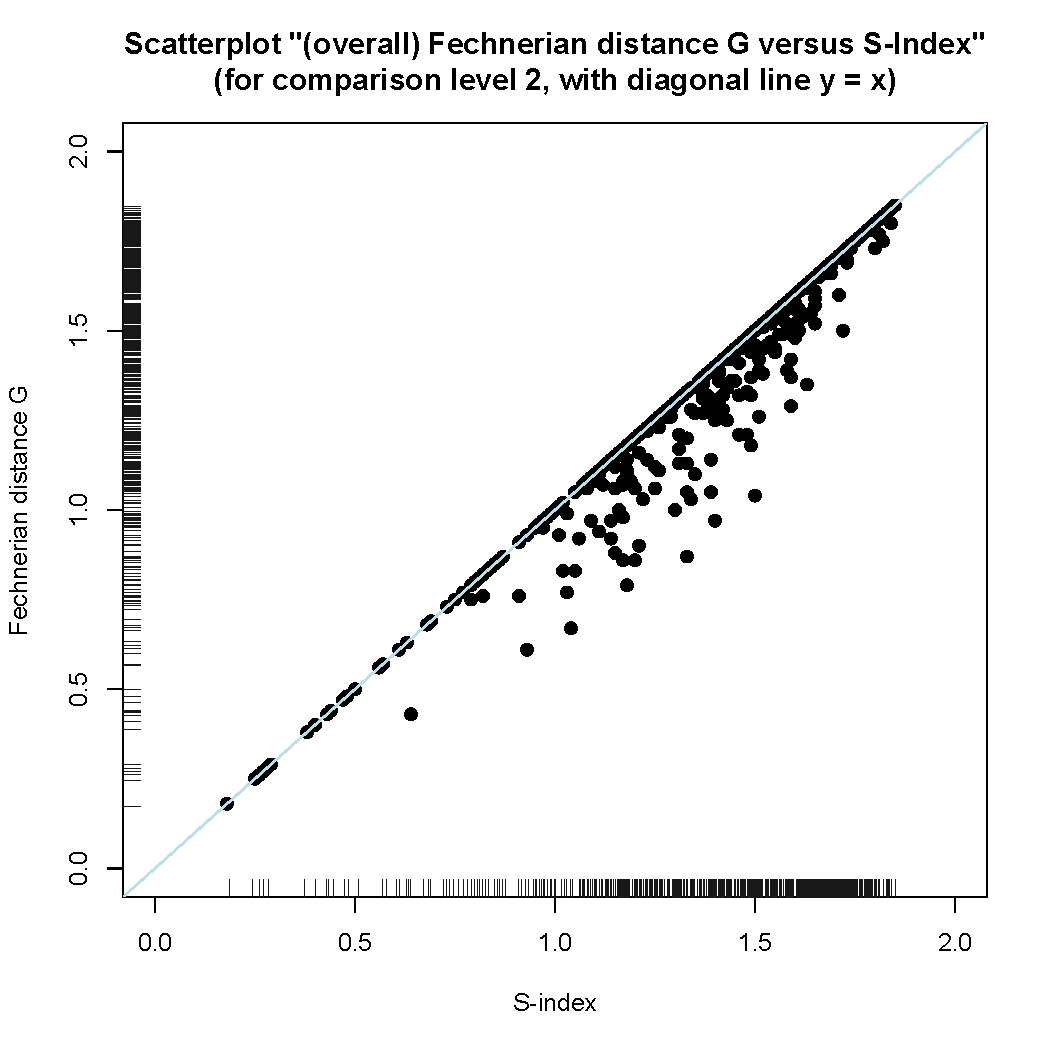
\includegraphics[scale=1]{fig3.pdf}
\caption{$G$ versus $S$--index for Morse code data (all stimuli pairs).}
\label{fig:3}
\end{center}
\end{figure}  

Objects of the class ``\code{fechner}'' can be plotted or summarized. Plotting the ``\code{fechner}'' object \code{f.scal.morse}
(computed based on the entire Morse code data set; see Section~\ref{subsec:regmin})
\begin{CodeChunk}
\begin{CodeInput}
R> plot(f.scal.morse)
\end{CodeInput}
\end{CodeChunk}
gives the scatterplot shown in Figure~\ref{fig:3}. 

Rugs are added to the axes and jittered (\code{amount = 0.01} of noise) to accommodate ties in the $S$--index and $G$ values.
The plot is for all (off-diagonal) pairs of stimuli (with geodesic loops containing at least $2$ links). If comparison is to involve 
only those $S$--index and $G$ values that have geodesic loops containing not less than $4$ links, the argument \code{level} must be set
$4$ (Figure~\ref{fig:4}):
\begin{CodeChunk}
\begin{CodeInput}
R> plot(f.scal.morse, level = 4)
\end{CodeInput}
\end{CodeChunk}

The corresponding summary of the ``\code{fechner}'' object \code{f.scal.morse}, 
including the Pearson correlation coefficient and the $C$--index:
\begin{CodeChunk}
\begin{CodeInput}
R> summary(f.scal.morse)
\end{CodeInput}
\begin{CodeOutput}
number of stimuli pairs used for comparison: 630 

summary of corresponding S-index values:
   Min. 1st Qu.  Median    Mean 3rd Qu.    Max. 
  0.180   1.260   1.520   1.435   1.670   1.850 

summary of corresponding Fechnerian distance G values:
   Min. 1st Qu.  Median    Mean 3rd Qu.    Max. 
  0.180   1.203   1.490   1.405   1.660   1.850 

Pearson correlation: 0.9764753 

C-index: 0.002925355 

comparison level: 2
\end{CodeOutput}
\end{CodeChunk}

In particular, detailed summary information can be accessed through assignment:
\begin{CodeChunk}
\begin{CodeInput}
R> detailed.summary.mo <- summary(f.scal.morse, level = 4)
R> str(detailed.summary.mo, vec.len = 2)
\end{CodeInput}
\begin{CodeOutput}
List of 4
 $ pairs.used.for.comparison:'data.frame':	63 obs. of  3 variables:
  ..$ stimuli.pairs        : chr [1:63] "B.J" "B.K" ...
  ..$ S.index              : num [1:63] 1.41 1.17 1.58 1.17 1.51 ...
  ..$ Fechnerian.distance.G: num [1:63] 1.28 0.86 1.39 0.98 1.44 ...
 $ Pearson.correlation      : num 0.87
 $ C.index                  : num 0.0219
 $ comparison.level         : num 4
 - attr(*, "class")= chr "summary.fechner"
\end{CodeOutput}
\end{CodeChunk}

\begin{figure}[t!]
\begin{center}
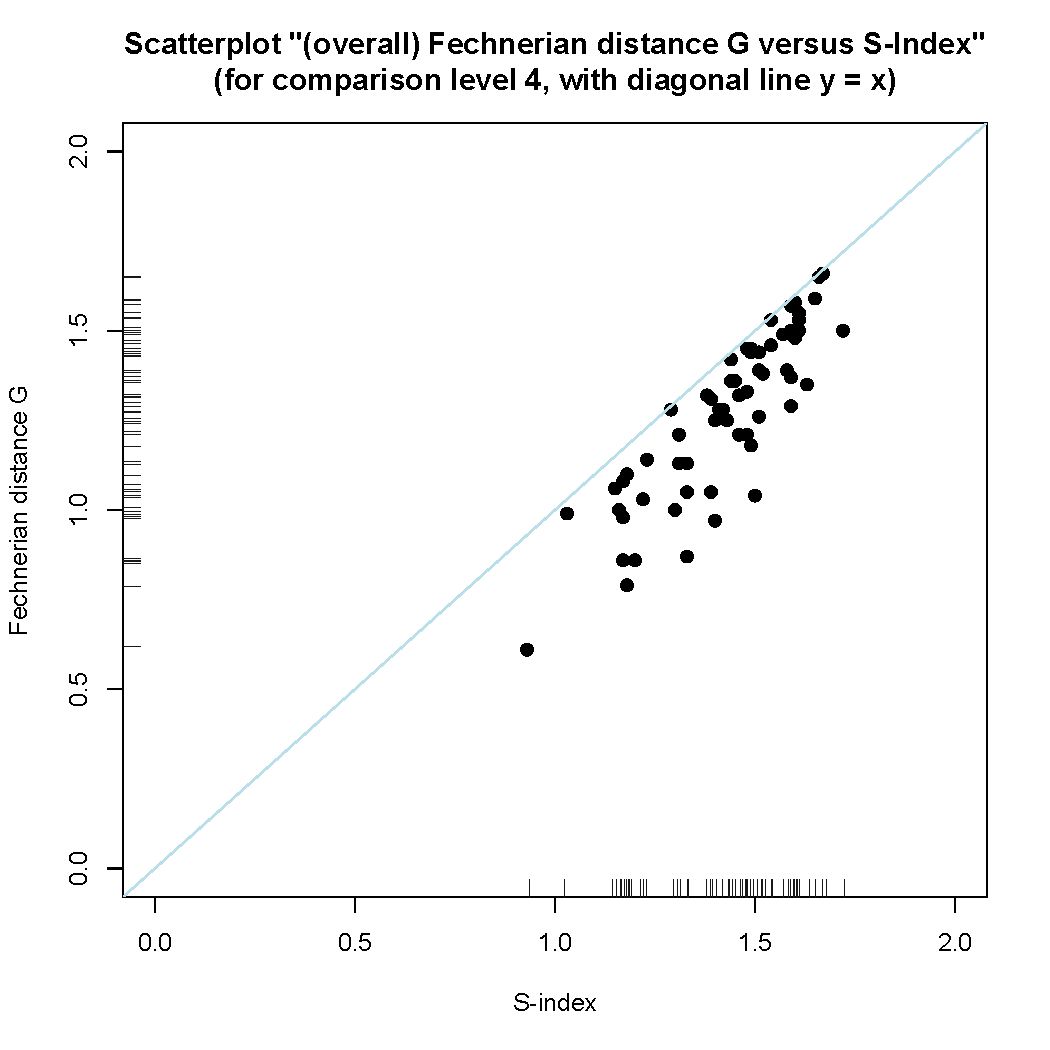
\includegraphics[scale=1]{fig4.pdf}
\caption{$G$ versus $S$--index for Morse code data (specific stimuli pairs).}
\label{fig:4}
\end{center}
\end{figure}  

For instance, the pair of stimuli $(B,J)$ and the corresponding $S$--index and $G$ values can be retrieved through:
\begin{CodeChunk}
\begin{CodeInput}
R> detailed.summary.mo$pairs.used.for.comparison[1, ]
\end{CodeInput}
\begin{CodeOutput}
  stimuli.pairs S.index Fechnerian.distance.G
1           B.J    1.41                  1.28
\end{CodeOutput}
\end{CodeChunk}
\pagebreak

To verify that obtained information:
\begin{CodeChunk}
\begin{CodeInput}
R> f.scal.morse$graph.lengths.of.geodesic.loops["B", "J"]
\end{CodeInput}
\begin{CodeOutput}
[1] 4
\end{CodeOutput}
\begin{CodeInput}
R> f.scal.morse$S.index["B", "J"]
\end{CodeInput}
\begin{CodeOutput}
[1] 1.41
\end{CodeOutput}
\begin{CodeInput}
R> f.scal.morse$overall.Fechnerian.distances["B", "J"]
\end{CodeInput}
\begin{CodeOutput}
[1] 1.28
\end{CodeOutput}
\end{CodeChunk}

\section{Conclusion} 
\label{sec:Concl}

We have introduced the package \pkg{fechner} for performing Fechnerian scaling (FS) of object sets in the \proglang{R} language 
and environment for statistical computing and graphics. The package has functions for checking the required data format and 
the regular minimality/maximality property, a fundamental property of discrimination in psychophysics. The main function 
of the package provides the FS computations, in the short and long variants. We have described the functions 
of the package \pkg{fechner} and demonstrated their usage on real and artificial data sets accompanying this package. 

By contributing the package \pkg{fechner} in \proglang{R} we hope to have established a basis for computational work in this field.
Interactive visualization and computational statistics approaches can be utilized in post-Fechnerian analyses to make the results 
obtained by FS (e.g., overall Fechnerian distances and geodesic loops) more explorable and interpretable. 
We plan to extend this package to incorporate such graphics as the matrix visualization, in particular combined with seriation, 
the fluctuation diagram variant of the mosaic plot, or the parallel coordinates plot---all as far as possible, interactively linked. 
(Available \proglang{R} packages providing for such graphics 
are, for example, \pkg{seriation}, \citealp{seriation}, and \pkg{iplots}, \citealp{iplots}.) These visualization approaches could be used in conjunction with post-Fechnerian 
analyses based on multidimensional scaling (MDS) or cluster analysis (CA), as described by \cite{DzhCol2006b}. 
Various MDS, dimensionality reduction, and CA techniques, as well as such methods as principal component analysis or factor analysis, 
are envisioned to be explored for their applicability to FS in greater depth.
The package \pkg{fechner} will have to be extended to incorporate such approaches.

The realization of FS in \proglang{R} may also prove valuable in applying current or conventional statistical methods 
to the theory of FS. 
For instance, the determination of confidence regions (e.g., for overall Fechnerian distances) and hypothesis testing (e.g., testing for RM) 
in FS are likely to be based on resampling methods. Such an endeavor would involve extensive computer simulation, something 
\proglang{R} would be ideally suited for.

\section*{Acknowledgments}

This research has been supported by NSF grant SES 0620446 and AFOSR grants FA9550-06-1-0288 and FA9550-09-1-0252 to Purdue University.
We thank two anonymous reviewers for their valuable comments that helped to improve the manuscript.

\bibliography{fechner}

\end{document}
